% Created by tikzDevice version 0.10.1 on 2017-12-04 15:15:14
% !TEX encoding = UTF-8 Unicode
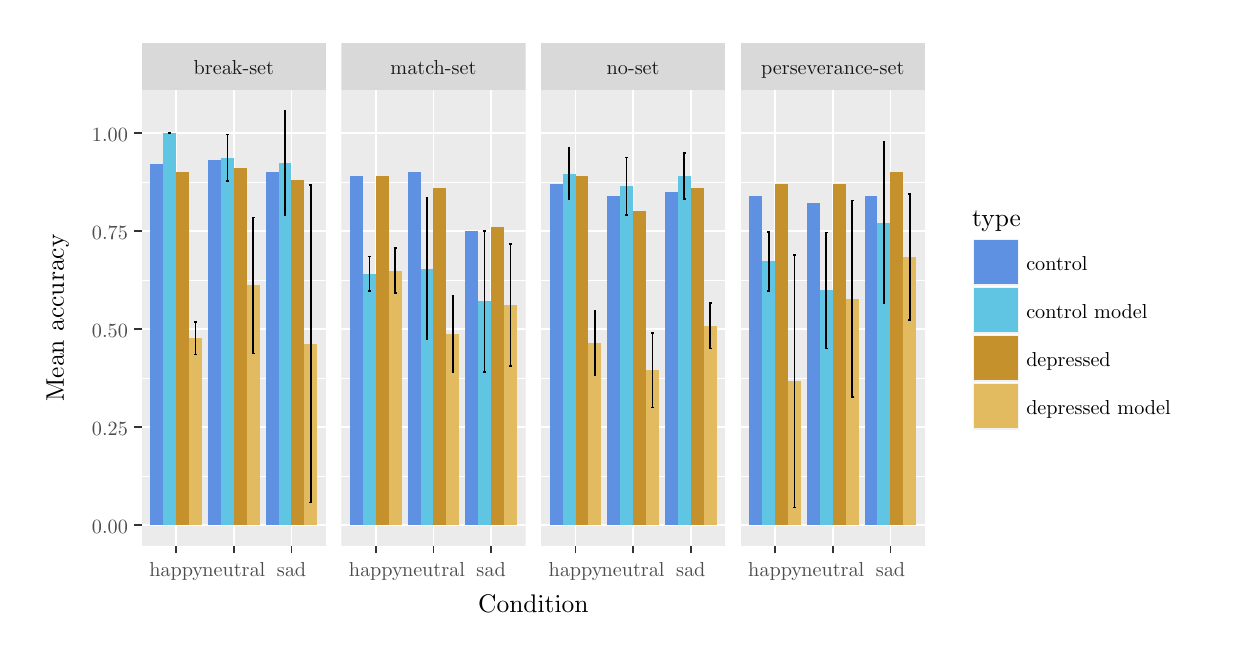
\begin{tikzpicture}[x=1pt,y=1pt]
\definecolor{fillColor}{RGB}{255,255,255}
\path[use as bounding box,fill=fillColor,fill opacity=0.00] (0,0) rectangle (433.62,216.81);
\begin{scope}
\path[clip] (  0.00,  0.00) rectangle (433.62,216.81);
\definecolor{drawColor}{RGB}{255,255,255}
\definecolor{fillColor}{RGB}{255,255,255}

\path[draw=drawColor,line width= 0.6pt,line join=round,line cap=round,fill=fillColor] (  0.00,  0.00) rectangle (433.62,216.81);
\end{scope}
\begin{scope}
\path[clip] ( 41.17, 29.59) rectangle (107.82,194.25);
\definecolor{fillColor}{gray}{0.92}

\path[fill=fillColor] ( 41.17, 29.59) rectangle (107.82,194.25);
\definecolor{drawColor}{RGB}{255,255,255}

\path[draw=drawColor,line width= 0.3pt,line join=round] ( 41.17, 54.79) --
	(107.82, 54.79);

\path[draw=drawColor,line width= 0.3pt,line join=round] ( 41.17, 90.21) --
	(107.82, 90.21);

\path[draw=drawColor,line width= 0.3pt,line join=round] ( 41.17,125.64) --
	(107.82,125.64);

\path[draw=drawColor,line width= 0.3pt,line join=round] ( 41.17,161.07) --
	(107.82,161.07);

\path[draw=drawColor,line width= 0.6pt,line join=round] ( 41.17, 37.07) --
	(107.82, 37.07);

\path[draw=drawColor,line width= 0.6pt,line join=round] ( 41.17, 72.50) --
	(107.82, 72.50);

\path[draw=drawColor,line width= 0.6pt,line join=round] ( 41.17,107.93) --
	(107.82,107.93);

\path[draw=drawColor,line width= 0.6pt,line join=round] ( 41.17,143.36) --
	(107.82,143.36);

\path[draw=drawColor,line width= 0.6pt,line join=round] ( 41.17,178.78) --
	(107.82,178.78);

\path[draw=drawColor,line width= 0.6pt,line join=round] ( 53.67, 29.59) --
	( 53.67,194.25);

\path[draw=drawColor,line width= 0.6pt,line join=round] ( 74.50, 29.59) --
	( 74.50,194.25);

\path[draw=drawColor,line width= 0.6pt,line join=round] ( 95.32, 29.59) --
	( 95.32,194.25);
\definecolor{fillColor}{RGB}{226,186,95}

\path[fill=fillColor] ( 58.36, 37.07) rectangle ( 63.04,104.55);
\definecolor{fillColor}{RGB}{196,145,45}

\path[fill=fillColor] ( 53.67, 37.07) rectangle ( 58.36,164.61);
\definecolor{fillColor}{RGB}{95,197,226}

\path[fill=fillColor] ( 48.98, 37.07) rectangle ( 53.67,178.78);
\definecolor{fillColor}{RGB}{95,145,226}

\path[fill=fillColor] ( 44.30, 37.07) rectangle ( 48.98,167.45);
\definecolor{fillColor}{RGB}{226,186,95}

\path[fill=fillColor] ( 79.18, 37.07) rectangle ( 83.87,123.67);
\definecolor{fillColor}{RGB}{196,145,45}

\path[fill=fillColor] ( 74.50, 37.07) rectangle ( 79.18,166.03);
\definecolor{fillColor}{RGB}{95,197,226}

\path[fill=fillColor] ( 69.81, 37.07) rectangle ( 74.50,169.85);
\definecolor{fillColor}{RGB}{95,145,226}

\path[fill=fillColor] ( 65.12, 37.07) rectangle ( 69.81,168.86);
\definecolor{fillColor}{RGB}{226,186,95}

\path[fill=fillColor] (100.01, 37.07) rectangle (104.69,102.56);
\definecolor{fillColor}{RGB}{196,145,45}

\path[fill=fillColor] ( 95.32, 37.07) rectangle (100.01,161.78);
\definecolor{fillColor}{RGB}{95,197,226}

\path[fill=fillColor] ( 90.64, 37.07) rectangle ( 95.32,167.88);
\definecolor{fillColor}{RGB}{95,145,226}

\path[fill=fillColor] ( 85.95, 37.07) rectangle ( 90.64,164.61);
\definecolor{drawColor}{RGB}{0,0,0}

\path[draw=drawColor,line width= 0.6pt,line join=round] ( 60.18,110.40) --
	( 61.22,110.40);

\path[draw=drawColor,line width= 0.6pt,line join=round] ( 60.70,110.40) --
	( 60.70, 98.71);

\path[draw=drawColor,line width= 0.6pt,line join=round] ( 60.18, 98.71) --
	( 61.22, 98.71);

\path[draw=drawColor,line width= 0.6pt,line join=round] ( 50.81,178.78) --
	( 51.85,178.78);

\path[draw=drawColor,line width= 0.6pt,line join=round] ( 51.33,178.78) --
	( 51.33,178.78);

\path[draw=drawColor,line width= 0.6pt,line join=round] ( 50.81,178.78) --
	( 51.85,178.78);

\path[draw=drawColor,line width= 0.6pt,line join=round] ( 81.00,148.26) --
	( 82.05,148.26);

\path[draw=drawColor,line width= 0.6pt,line join=round] ( 81.52,148.26) --
	( 81.52, 99.09);

\path[draw=drawColor,line width= 0.6pt,line join=round] ( 81.00, 99.09) --
	( 82.05, 99.09);

\path[draw=drawColor,line width= 0.6pt,line join=round] ( 71.63,178.25) --
	( 72.67,178.25);

\path[draw=drawColor,line width= 0.6pt,line join=round] ( 72.15,178.25) --
	( 72.15,161.45);

\path[draw=drawColor,line width= 0.6pt,line join=round] ( 71.63,161.45) --
	( 72.67,161.45);

\path[draw=drawColor,line width= 0.6pt,line join=round] (101.83,159.84) --
	(102.87,159.84);

\path[draw=drawColor,line width= 0.6pt,line join=round] (102.35,159.84) --
	(102.35, 45.28);

\path[draw=drawColor,line width= 0.6pt,line join=round] (101.83, 45.28) --
	(102.87, 45.28);

\path[draw=drawColor,line width= 0.6pt,line join=round] ( 92.46,186.76) --
	( 93.50,186.76);

\path[draw=drawColor,line width= 0.6pt,line join=round] ( 92.98,186.76) --
	( 92.98,149.00);

\path[draw=drawColor,line width= 0.6pt,line join=round] ( 92.46,149.00) --
	( 93.50,149.00);
\end{scope}
\begin{scope}
\path[clip] (113.32, 29.59) rectangle (179.96,194.25);
\definecolor{fillColor}{gray}{0.92}

\path[fill=fillColor] (113.32, 29.59) rectangle (179.96,194.25);
\definecolor{drawColor}{RGB}{255,255,255}

\path[draw=drawColor,line width= 0.3pt,line join=round] (113.32, 54.79) --
	(179.96, 54.79);

\path[draw=drawColor,line width= 0.3pt,line join=round] (113.32, 90.21) --
	(179.96, 90.21);

\path[draw=drawColor,line width= 0.3pt,line join=round] (113.32,125.64) --
	(179.96,125.64);

\path[draw=drawColor,line width= 0.3pt,line join=round] (113.32,161.07) --
	(179.96,161.07);

\path[draw=drawColor,line width= 0.6pt,line join=round] (113.32, 37.07) --
	(179.96, 37.07);

\path[draw=drawColor,line width= 0.6pt,line join=round] (113.32, 72.50) --
	(179.96, 72.50);

\path[draw=drawColor,line width= 0.6pt,line join=round] (113.32,107.93) --
	(179.96,107.93);

\path[draw=drawColor,line width= 0.6pt,line join=round] (113.32,143.36) --
	(179.96,143.36);

\path[draw=drawColor,line width= 0.6pt,line join=round] (113.32,178.78) --
	(179.96,178.78);

\path[draw=drawColor,line width= 0.6pt,line join=round] (125.81, 29.59) --
	(125.81,194.25);

\path[draw=drawColor,line width= 0.6pt,line join=round] (146.64, 29.59) --
	(146.64,194.25);

\path[draw=drawColor,line width= 0.6pt,line join=round] (167.47, 29.59) --
	(167.47,194.25);
\definecolor{fillColor}{RGB}{226,186,95}

\path[fill=fillColor] (130.50, 37.07) rectangle (135.19,129.03);
\definecolor{fillColor}{RGB}{196,145,45}

\path[fill=fillColor] (125.81, 37.07) rectangle (130.50,163.20);
\definecolor{fillColor}{RGB}{95,197,226}

\path[fill=fillColor] (121.13, 37.07) rectangle (125.81,127.95);
\definecolor{fillColor}{RGB}{95,145,226}

\path[fill=fillColor] (116.44, 37.07) rectangle (121.13,163.20);
\definecolor{fillColor}{RGB}{226,186,95}

\path[fill=fillColor] (151.33, 37.07) rectangle (156.01,106.21);
\definecolor{fillColor}{RGB}{196,145,45}

\path[fill=fillColor] (146.64, 37.07) rectangle (151.33,158.94);
\definecolor{fillColor}{RGB}{95,197,226}

\path[fill=fillColor] (141.95, 37.07) rectangle (146.64,129.69);
\definecolor{fillColor}{RGB}{95,145,226}

\path[fill=fillColor] (137.27, 37.07) rectangle (141.95,164.61);
\definecolor{fillColor}{RGB}{226,186,95}

\path[fill=fillColor] (172.15, 37.07) rectangle (176.84,116.52);
\definecolor{fillColor}{RGB}{196,145,45}

\path[fill=fillColor] (167.47, 37.07) rectangle (172.15,144.77);
\definecolor{fillColor}{RGB}{95,197,226}

\path[fill=fillColor] (162.78, 37.07) rectangle (167.47,117.96);
\definecolor{fillColor}{RGB}{95,145,226}

\path[fill=fillColor] (158.10, 37.07) rectangle (162.78,143.36);
\definecolor{drawColor}{RGB}{0,0,0}

\path[draw=drawColor,line width= 0.6pt,line join=round] (132.32,137.18) --
	(133.36,137.18);

\path[draw=drawColor,line width= 0.6pt,line join=round] (132.84,137.18) --
	(132.84,120.89);

\path[draw=drawColor,line width= 0.6pt,line join=round] (132.32,120.89) --
	(133.36,120.89);

\path[draw=drawColor,line width= 0.6pt,line join=round] (122.95,134.18) --
	(123.99,134.18);

\path[draw=drawColor,line width= 0.6pt,line join=round] (123.47,134.18) --
	(123.47,121.72);

\path[draw=drawColor,line width= 0.6pt,line join=round] (122.95,121.72) --
	(123.99,121.72);

\path[draw=drawColor,line width= 0.6pt,line join=round] (153.15,120.06) --
	(154.19,120.06);

\path[draw=drawColor,line width= 0.6pt,line join=round] (153.67,120.06) --
	(153.67, 92.36);

\path[draw=drawColor,line width= 0.6pt,line join=round] (153.15, 92.36) --
	(154.19, 92.36);

\path[draw=drawColor,line width= 0.6pt,line join=round] (143.78,155.28) --
	(144.82,155.28);

\path[draw=drawColor,line width= 0.6pt,line join=round] (144.30,155.28) --
	(144.30,104.10);

\path[draw=drawColor,line width= 0.6pt,line join=round] (143.78,104.10) --
	(144.82,104.10);

\path[draw=drawColor,line width= 0.6pt,line join=round] (173.98,138.57) --
	(175.02,138.57);

\path[draw=drawColor,line width= 0.6pt,line join=round] (174.50,138.57) --
	(174.50, 94.46);

\path[draw=drawColor,line width= 0.6pt,line join=round] (173.98, 94.46) --
	(175.02, 94.46);

\path[draw=drawColor,line width= 0.6pt,line join=round] (164.60,143.43) --
	(165.64,143.43);

\path[draw=drawColor,line width= 0.6pt,line join=round] (165.12,143.43) --
	(165.12, 92.49);

\path[draw=drawColor,line width= 0.6pt,line join=round] (164.60, 92.49) --
	(165.64, 92.49);
\end{scope}
\begin{scope}
\path[clip] (185.46, 29.59) rectangle (252.11,194.25);
\definecolor{fillColor}{gray}{0.92}

\path[fill=fillColor] (185.46, 29.59) rectangle (252.11,194.25);
\definecolor{drawColor}{RGB}{255,255,255}

\path[draw=drawColor,line width= 0.3pt,line join=round] (185.46, 54.79) --
	(252.11, 54.79);

\path[draw=drawColor,line width= 0.3pt,line join=round] (185.46, 90.21) --
	(252.11, 90.21);

\path[draw=drawColor,line width= 0.3pt,line join=round] (185.46,125.64) --
	(252.11,125.64);

\path[draw=drawColor,line width= 0.3pt,line join=round] (185.46,161.07) --
	(252.11,161.07);

\path[draw=drawColor,line width= 0.6pt,line join=round] (185.46, 37.07) --
	(252.11, 37.07);

\path[draw=drawColor,line width= 0.6pt,line join=round] (185.46, 72.50) --
	(252.11, 72.50);

\path[draw=drawColor,line width= 0.6pt,line join=round] (185.46,107.93) --
	(252.11,107.93);

\path[draw=drawColor,line width= 0.6pt,line join=round] (185.46,143.36) --
	(252.11,143.36);

\path[draw=drawColor,line width= 0.6pt,line join=round] (185.46,178.78) --
	(252.11,178.78);

\path[draw=drawColor,line width= 0.6pt,line join=round] (197.96, 29.59) --
	(197.96,194.25);

\path[draw=drawColor,line width= 0.6pt,line join=round] (218.79, 29.59) --
	(218.79,194.25);

\path[draw=drawColor,line width= 0.6pt,line join=round] (239.61, 29.59) --
	(239.61,194.25);
\definecolor{fillColor}{RGB}{226,186,95}

\path[fill=fillColor] (202.64, 37.07) rectangle (207.33,102.75);
\definecolor{fillColor}{RGB}{196,145,45}

\path[fill=fillColor] (197.96, 37.07) rectangle (202.64,163.20);
\definecolor{fillColor}{RGB}{95,197,226}

\path[fill=fillColor] (193.27, 37.07) rectangle (197.96,163.98);
\definecolor{fillColor}{RGB}{95,145,226}

\path[fill=fillColor] (188.59, 37.07) rectangle (193.27,160.36);
\definecolor{fillColor}{RGB}{226,186,95}

\path[fill=fillColor] (223.47, 37.07) rectangle (228.16, 93.04);
\definecolor{fillColor}{RGB}{196,145,45}

\path[fill=fillColor] (218.79, 37.07) rectangle (223.47,150.44);
\definecolor{fillColor}{RGB}{95,197,226}

\path[fill=fillColor] (214.10, 37.07) rectangle (218.79,159.45);
\definecolor{fillColor}{RGB}{95,145,226}

\path[fill=fillColor] (209.41, 37.07) rectangle (214.10,156.11);
\definecolor{fillColor}{RGB}{226,186,95}

\path[fill=fillColor] (244.30, 37.07) rectangle (248.98,109.11);
\definecolor{fillColor}{RGB}{196,145,45}

\path[fill=fillColor] (239.61, 37.07) rectangle (244.30,158.94);
\definecolor{fillColor}{RGB}{95,197,226}

\path[fill=fillColor] (234.93, 37.07) rectangle (239.61,163.25);
\definecolor{fillColor}{RGB}{95,145,226}

\path[fill=fillColor] (230.24, 37.07) rectangle (234.93,157.53);
\definecolor{drawColor}{RGB}{0,0,0}

\path[draw=drawColor,line width= 0.6pt,line join=round] (204.47,114.32) --
	(205.51,114.32);

\path[draw=drawColor,line width= 0.6pt,line join=round] (204.99,114.32) --
	(204.99, 91.18);

\path[draw=drawColor,line width= 0.6pt,line join=round] (204.47, 91.18) --
	(205.51, 91.18);

\path[draw=drawColor,line width= 0.6pt,line join=round] (195.10,173.26) --
	(196.14,173.26);

\path[draw=drawColor,line width= 0.6pt,line join=round] (195.62,173.26) --
	(195.62,154.69);

\path[draw=drawColor,line width= 0.6pt,line join=round] (195.10,154.69) --
	(196.14,154.69);

\path[draw=drawColor,line width= 0.6pt,line join=round] (225.29,106.55) --
	(226.34,106.55);

\path[draw=drawColor,line width= 0.6pt,line join=round] (225.81,106.55) --
	(225.81, 79.53);

\path[draw=drawColor,line width= 0.6pt,line join=round] (225.29, 79.53) --
	(226.34, 79.53);

\path[draw=drawColor,line width= 0.6pt,line join=round] (215.92,169.90) --
	(216.96,169.90);

\path[draw=drawColor,line width= 0.6pt,line join=round] (216.44,169.90) --
	(216.44,149.00);

\path[draw=drawColor,line width= 0.6pt,line join=round] (215.92,149.00) --
	(216.96,149.00);

\path[draw=drawColor,line width= 0.6pt,line join=round] (246.12,117.38) --
	(247.16,117.38);

\path[draw=drawColor,line width= 0.6pt,line join=round] (246.64,117.38) --
	(246.64,100.84);

\path[draw=drawColor,line width= 0.6pt,line join=round] (246.12,100.84) --
	(247.16,100.84);

\path[draw=drawColor,line width= 0.6pt,line join=round] (236.75,171.52) --
	(237.79,171.52);

\path[draw=drawColor,line width= 0.6pt,line join=round] (237.27,171.52) --
	(237.27,154.98);

\path[draw=drawColor,line width= 0.6pt,line join=round] (236.75,154.98) --
	(237.79,154.98);
\end{scope}
\begin{scope}
\path[clip] (257.61, 29.59) rectangle (324.25,194.25);
\definecolor{fillColor}{gray}{0.92}

\path[fill=fillColor] (257.61, 29.59) rectangle (324.25,194.25);
\definecolor{drawColor}{RGB}{255,255,255}

\path[draw=drawColor,line width= 0.3pt,line join=round] (257.61, 54.79) --
	(324.25, 54.79);

\path[draw=drawColor,line width= 0.3pt,line join=round] (257.61, 90.21) --
	(324.25, 90.21);

\path[draw=drawColor,line width= 0.3pt,line join=round] (257.61,125.64) --
	(324.25,125.64);

\path[draw=drawColor,line width= 0.3pt,line join=round] (257.61,161.07) --
	(324.25,161.07);

\path[draw=drawColor,line width= 0.6pt,line join=round] (257.61, 37.07) --
	(324.25, 37.07);

\path[draw=drawColor,line width= 0.6pt,line join=round] (257.61, 72.50) --
	(324.25, 72.50);

\path[draw=drawColor,line width= 0.6pt,line join=round] (257.61,107.93) --
	(324.25,107.93);

\path[draw=drawColor,line width= 0.6pt,line join=round] (257.61,143.36) --
	(324.25,143.36);

\path[draw=drawColor,line width= 0.6pt,line join=round] (257.61,178.78) --
	(324.25,178.78);

\path[draw=drawColor,line width= 0.6pt,line join=round] (270.10, 29.59) --
	(270.10,194.25);

\path[draw=drawColor,line width= 0.6pt,line join=round] (290.93, 29.59) --
	(290.93,194.25);

\path[draw=drawColor,line width= 0.6pt,line join=round] (311.76, 29.59) --
	(311.76,194.25);
\definecolor{fillColor}{RGB}{226,186,95}

\path[fill=fillColor] (274.79, 37.07) rectangle (279.48, 89.03);
\definecolor{fillColor}{RGB}{196,145,45}

\path[fill=fillColor] (270.10, 37.07) rectangle (274.79,160.36);
\definecolor{fillColor}{RGB}{95,197,226}

\path[fill=fillColor] (265.42, 37.07) rectangle (270.10,132.33);
\definecolor{fillColor}{RGB}{95,145,226}

\path[fill=fillColor] (260.73, 37.07) rectangle (265.42,156.11);
\definecolor{fillColor}{RGB}{226,186,95}

\path[fill=fillColor] (295.62, 37.07) rectangle (300.30,118.89);
\definecolor{fillColor}{RGB}{196,145,45}

\path[fill=fillColor] (290.93, 37.07) rectangle (295.62,160.36);
\definecolor{fillColor}{RGB}{95,197,226}

\path[fill=fillColor] (286.24, 37.07) rectangle (290.93,121.87);
\definecolor{fillColor}{RGB}{95,145,226}

\path[fill=fillColor] (281.56, 37.07) rectangle (286.24,153.28);
\definecolor{fillColor}{RGB}{226,186,95}

\path[fill=fillColor] (316.44, 37.07) rectangle (321.13,133.91);
\definecolor{fillColor}{RGB}{196,145,45}

\path[fill=fillColor] (311.76, 37.07) rectangle (316.44,164.61);
\definecolor{fillColor}{RGB}{95,197,226}

\path[fill=fillColor] (307.07, 37.07) rectangle (311.76,146.39);
\definecolor{fillColor}{RGB}{95,145,226}

\path[fill=fillColor] (302.39, 37.07) rectangle (307.07,156.11);
\definecolor{drawColor}{RGB}{0,0,0}

\path[draw=drawColor,line width= 0.6pt,line join=round] (276.61,134.59) --
	(277.65,134.59);

\path[draw=drawColor,line width= 0.6pt,line join=round] (277.13,134.59) --
	(277.13, 43.48);

\path[draw=drawColor,line width= 0.6pt,line join=round] (276.61, 43.48) --
	(277.65, 43.48);

\path[draw=drawColor,line width= 0.6pt,line join=round] (267.24,142.98) --
	(268.28,142.98);

\path[draw=drawColor,line width= 0.6pt,line join=round] (267.76,142.98) --
	(267.76,121.68);

\path[draw=drawColor,line width= 0.6pt,line join=round] (267.24,121.68) --
	(268.28,121.68);

\path[draw=drawColor,line width= 0.6pt,line join=round] (297.44,154.35) --
	(298.48,154.35);

\path[draw=drawColor,line width= 0.6pt,line join=round] (297.96,154.35) --
	(297.96, 83.44);

\path[draw=drawColor,line width= 0.6pt,line join=round] (297.44, 83.44) --
	(298.48, 83.44);

\path[draw=drawColor,line width= 0.6pt,line join=round] (288.07,142.85) --
	(289.11,142.85);

\path[draw=drawColor,line width= 0.6pt,line join=round] (288.59,142.85) --
	(288.59,100.90);

\path[draw=drawColor,line width= 0.6pt,line join=round] (288.07,100.90) --
	(289.11,100.90);

\path[draw=drawColor,line width= 0.6pt,line join=round] (318.27,156.69) --
	(319.31,156.69);

\path[draw=drawColor,line width= 0.6pt,line join=round] (318.79,156.69) --
	(318.79,111.13);

\path[draw=drawColor,line width= 0.6pt,line join=round] (318.27,111.13) --
	(319.31,111.13);

\path[draw=drawColor,line width= 0.6pt,line join=round] (308.89,175.59) --
	(309.93,175.59);

\path[draw=drawColor,line width= 0.6pt,line join=round] (309.41,175.59) --
	(309.41,117.20);

\path[draw=drawColor,line width= 0.6pt,line join=round] (308.89,117.20) --
	(309.93,117.20);
\end{scope}
\begin{scope}
\path[clip] ( 41.17,194.25) rectangle (107.82,211.31);
\definecolor{fillColor}{gray}{0.85}

\path[fill=fillColor] ( 41.17,194.25) rectangle (107.82,211.31);
\definecolor{drawColor}{gray}{0.10}

\node[text=drawColor,anchor=base,inner sep=0pt, outer sep=0pt, scale=  0.73] at ( 74.50,199.75) {break-set};
\end{scope}
\begin{scope}
\path[clip] (113.32,194.25) rectangle (179.96,211.31);
\definecolor{fillColor}{gray}{0.85}

\path[fill=fillColor] (113.32,194.25) rectangle (179.96,211.31);
\definecolor{drawColor}{gray}{0.10}

\node[text=drawColor,anchor=base,inner sep=0pt, outer sep=0pt, scale=  0.73] at (146.64,199.75) {match-set};
\end{scope}
\begin{scope}
\path[clip] (185.46,194.25) rectangle (252.11,211.31);
\definecolor{fillColor}{gray}{0.85}

\path[fill=fillColor] (185.46,194.25) rectangle (252.11,211.31);
\definecolor{drawColor}{gray}{0.10}

\node[text=drawColor,anchor=base,inner sep=0pt, outer sep=0pt, scale=  0.73] at (218.79,199.75) {no-set};
\end{scope}
\begin{scope}
\path[clip] (257.61,194.25) rectangle (324.25,211.31);
\definecolor{fillColor}{gray}{0.85}

\path[fill=fillColor] (257.61,194.25) rectangle (324.25,211.31);
\definecolor{drawColor}{gray}{0.10}

\node[text=drawColor,anchor=base,inner sep=0pt, outer sep=0pt, scale=  0.73] at (290.93,199.75) {perseverance-set};
\end{scope}
\begin{scope}
\path[clip] (  0.00,  0.00) rectangle (433.62,216.81);
\definecolor{drawColor}{gray}{0.20}

\path[draw=drawColor,line width= 0.6pt,line join=round] ( 53.67, 26.84) --
	( 53.67, 29.59);

\path[draw=drawColor,line width= 0.6pt,line join=round] ( 74.50, 26.84) --
	( 74.50, 29.59);

\path[draw=drawColor,line width= 0.6pt,line join=round] ( 95.32, 26.84) --
	( 95.32, 29.59);
\end{scope}
\begin{scope}
\path[clip] (  0.00,  0.00) rectangle (433.62,216.81);
\definecolor{drawColor}{gray}{0.30}

\node[text=drawColor,anchor=base,inner sep=0pt, outer sep=0pt, scale=  0.73] at ( 53.67, 18.58) {happy};

\node[text=drawColor,anchor=base,inner sep=0pt, outer sep=0pt, scale=  0.73] at ( 74.50, 18.58) {neutral};

\node[text=drawColor,anchor=base,inner sep=0pt, outer sep=0pt, scale=  0.73] at ( 95.32, 18.58) {sad};
\end{scope}
\begin{scope}
\path[clip] (  0.00,  0.00) rectangle (433.62,216.81);
\definecolor{drawColor}{gray}{0.20}

\path[draw=drawColor,line width= 0.6pt,line join=round] (125.81, 26.84) --
	(125.81, 29.59);

\path[draw=drawColor,line width= 0.6pt,line join=round] (146.64, 26.84) --
	(146.64, 29.59);

\path[draw=drawColor,line width= 0.6pt,line join=round] (167.47, 26.84) --
	(167.47, 29.59);
\end{scope}
\begin{scope}
\path[clip] (  0.00,  0.00) rectangle (433.62,216.81);
\definecolor{drawColor}{gray}{0.30}

\node[text=drawColor,anchor=base,inner sep=0pt, outer sep=0pt, scale=  0.73] at (125.81, 18.58) {happy};

\node[text=drawColor,anchor=base,inner sep=0pt, outer sep=0pt, scale=  0.73] at (146.64, 18.58) {neutral};

\node[text=drawColor,anchor=base,inner sep=0pt, outer sep=0pt, scale=  0.73] at (167.47, 18.58) {sad};
\end{scope}
\begin{scope}
\path[clip] (  0.00,  0.00) rectangle (433.62,216.81);
\definecolor{drawColor}{gray}{0.20}

\path[draw=drawColor,line width= 0.6pt,line join=round] (197.96, 26.84) --
	(197.96, 29.59);

\path[draw=drawColor,line width= 0.6pt,line join=round] (218.79, 26.84) --
	(218.79, 29.59);

\path[draw=drawColor,line width= 0.6pt,line join=round] (239.61, 26.84) --
	(239.61, 29.59);
\end{scope}
\begin{scope}
\path[clip] (  0.00,  0.00) rectangle (433.62,216.81);
\definecolor{drawColor}{gray}{0.30}

\node[text=drawColor,anchor=base,inner sep=0pt, outer sep=0pt, scale=  0.73] at (197.96, 18.58) {happy};

\node[text=drawColor,anchor=base,inner sep=0pt, outer sep=0pt, scale=  0.73] at (218.79, 18.58) {neutral};

\node[text=drawColor,anchor=base,inner sep=0pt, outer sep=0pt, scale=  0.73] at (239.61, 18.58) {sad};
\end{scope}
\begin{scope}
\path[clip] (  0.00,  0.00) rectangle (433.62,216.81);
\definecolor{drawColor}{gray}{0.20}

\path[draw=drawColor,line width= 0.6pt,line join=round] (270.10, 26.84) --
	(270.10, 29.59);

\path[draw=drawColor,line width= 0.6pt,line join=round] (290.93, 26.84) --
	(290.93, 29.59);

\path[draw=drawColor,line width= 0.6pt,line join=round] (311.76, 26.84) --
	(311.76, 29.59);
\end{scope}
\begin{scope}
\path[clip] (  0.00,  0.00) rectangle (433.62,216.81);
\definecolor{drawColor}{gray}{0.30}

\node[text=drawColor,anchor=base,inner sep=0pt, outer sep=0pt, scale=  0.73] at (270.10, 18.58) {happy};

\node[text=drawColor,anchor=base,inner sep=0pt, outer sep=0pt, scale=  0.73] at (290.93, 18.58) {neutral};

\node[text=drawColor,anchor=base,inner sep=0pt, outer sep=0pt, scale=  0.73] at (311.76, 18.58) {sad};
\end{scope}
\begin{scope}
\path[clip] (  0.00,  0.00) rectangle (433.62,216.81);
\definecolor{drawColor}{gray}{0.30}

\node[text=drawColor,anchor=base east,inner sep=0pt, outer sep=0pt, scale=  0.73] at ( 36.22, 34.04) {0.00};

\node[text=drawColor,anchor=base east,inner sep=0pt, outer sep=0pt, scale=  0.73] at ( 36.22, 69.47) {0.25};

\node[text=drawColor,anchor=base east,inner sep=0pt, outer sep=0pt, scale=  0.73] at ( 36.22,104.90) {0.50};

\node[text=drawColor,anchor=base east,inner sep=0pt, outer sep=0pt, scale=  0.73] at ( 36.22,140.33) {0.75};

\node[text=drawColor,anchor=base east,inner sep=0pt, outer sep=0pt, scale=  0.73] at ( 36.22,175.75) {1.00};
\end{scope}
\begin{scope}
\path[clip] (  0.00,  0.00) rectangle (433.62,216.81);
\definecolor{drawColor}{gray}{0.20}

\path[draw=drawColor,line width= 0.6pt,line join=round] ( 38.42, 37.07) --
	( 41.17, 37.07);

\path[draw=drawColor,line width= 0.6pt,line join=round] ( 38.42, 72.50) --
	( 41.17, 72.50);

\path[draw=drawColor,line width= 0.6pt,line join=round] ( 38.42,107.93) --
	( 41.17,107.93);

\path[draw=drawColor,line width= 0.6pt,line join=round] ( 38.42,143.36) --
	( 41.17,143.36);

\path[draw=drawColor,line width= 0.6pt,line join=round] ( 38.42,178.78) --
	( 41.17,178.78);
\end{scope}
\begin{scope}
\path[clip] (  0.00,  0.00) rectangle (433.62,216.81);
\definecolor{drawColor}{RGB}{0,0,0}

\node[text=drawColor,anchor=base,inner sep=0pt, outer sep=0pt, scale=  0.92] at (182.71,  5.50) {Condition};
\end{scope}
\begin{scope}
\path[clip] (  0.00,  0.00) rectangle (433.62,216.81);
\definecolor{drawColor}{RGB}{0,0,0}

\node[text=drawColor,rotate= 90.00,anchor=base,inner sep=0pt, outer sep=0pt, scale=  0.92] at ( 13.08,111.92) {Mean accuracy};
\end{scope}
\begin{scope}
\path[clip] (  0.00,  0.00) rectangle (433.62,216.81);
\definecolor{fillColor}{RGB}{255,255,255}

\path[fill=fillColor] (335.63, 65.58) rectangle (428.12,158.25);
\end{scope}
\begin{scope}
\path[clip] (  0.00,  0.00) rectangle (433.62,216.81);
\definecolor{drawColor}{RGB}{0,0,0}

\node[text=drawColor,anchor=base west,inner sep=0pt, outer sep=0pt, scale=  0.92] at (341.32,144.99) {type};
\end{scope}
\begin{scope}
\path[clip] (  0.00,  0.00) rectangle (433.62,216.81);
\definecolor{drawColor}{RGB}{255,255,255}
\definecolor{fillColor}{gray}{0.95}

\path[draw=drawColor,line width= 0.6pt,line join=round,line cap=round,fill=fillColor] (341.32,123.31) rectangle (358.67,140.65);
\end{scope}
\begin{scope}
\path[clip] (  0.00,  0.00) rectangle (433.62,216.81);
\definecolor{fillColor}{RGB}{95,145,226}

\path[fill=fillColor] (342.04,124.02) rectangle (357.96,139.94);
\end{scope}
\begin{scope}
\path[clip] (  0.00,  0.00) rectangle (433.62,216.81);
\definecolor{drawColor}{RGB}{255,255,255}
\definecolor{fillColor}{gray}{0.95}

\path[draw=drawColor,line width= 0.6pt,line join=round,line cap=round,fill=fillColor] (341.32,105.96) rectangle (358.67,123.31);
\end{scope}
\begin{scope}
\path[clip] (  0.00,  0.00) rectangle (433.62,216.81);
\definecolor{fillColor}{RGB}{95,197,226}

\path[fill=fillColor] (342.04,106.67) rectangle (357.96,122.60);
\end{scope}
\begin{scope}
\path[clip] (  0.00,  0.00) rectangle (433.62,216.81);
\definecolor{drawColor}{RGB}{255,255,255}
\definecolor{fillColor}{gray}{0.95}

\path[draw=drawColor,line width= 0.6pt,line join=round,line cap=round,fill=fillColor] (341.32, 88.62) rectangle (358.67,105.96);
\end{scope}
\begin{scope}
\path[clip] (  0.00,  0.00) rectangle (433.62,216.81);
\definecolor{fillColor}{RGB}{196,145,45}

\path[fill=fillColor] (342.04, 89.33) rectangle (357.96,105.25);
\end{scope}
\begin{scope}
\path[clip] (  0.00,  0.00) rectangle (433.62,216.81);
\definecolor{drawColor}{RGB}{255,255,255}
\definecolor{fillColor}{gray}{0.95}

\path[draw=drawColor,line width= 0.6pt,line join=round,line cap=round,fill=fillColor] (341.32, 71.27) rectangle (358.67, 88.62);
\end{scope}
\begin{scope}
\path[clip] (  0.00,  0.00) rectangle (433.62,216.81);
\definecolor{fillColor}{RGB}{226,186,95}

\path[fill=fillColor] (342.04, 71.98) rectangle (357.96, 87.91);
\end{scope}
\begin{scope}
\path[clip] (  0.00,  0.00) rectangle (433.62,216.81);
\definecolor{drawColor}{RGB}{0,0,0}

\node[text=drawColor,anchor=base west,inner sep=0pt, outer sep=0pt, scale=  0.73] at (360.84,128.95) {control};
\end{scope}
\begin{scope}
\path[clip] (  0.00,  0.00) rectangle (433.62,216.81);
\definecolor{drawColor}{RGB}{0,0,0}

\node[text=drawColor,anchor=base west,inner sep=0pt, outer sep=0pt, scale=  0.73] at (360.84,111.60) {control model};
\end{scope}
\begin{scope}
\path[clip] (  0.00,  0.00) rectangle (433.62,216.81);
\definecolor{drawColor}{RGB}{0,0,0}

\node[text=drawColor,anchor=base west,inner sep=0pt, outer sep=0pt, scale=  0.73] at (360.84, 94.26) {depressed};
\end{scope}
\begin{scope}
\path[clip] (  0.00,  0.00) rectangle (433.62,216.81);
\definecolor{drawColor}{RGB}{0,0,0}

\node[text=drawColor,anchor=base west,inner sep=0pt, outer sep=0pt, scale=  0.73] at (360.84, 76.91) {depressed model};
\end{scope}
\end{tikzpicture}
